\chapter{Fonction inverse}
\section{Fonction inverse}

\begin{definition}
  La fonction définie sur $\mathbb R^*$ par $f(x)=\frac{1}{x}$ est appelée \emph{fonction inverse}.
\end{definition}

\begin{propriete}[Variations]
  Le tableau de variations de la fonction inverse est :
  \begin{center}
    \begin{tikzpicture}
      \tkzTabInit[lgt=2,espcl=2]
      {$x$ /1,
        $\dfrac{1}{x}$ /2}
      {$-\infty$,$0$,$+\infty$}%
      \tkzTabVar{+/, -D+//, -/}
    \end{tikzpicture}
    \hfill
  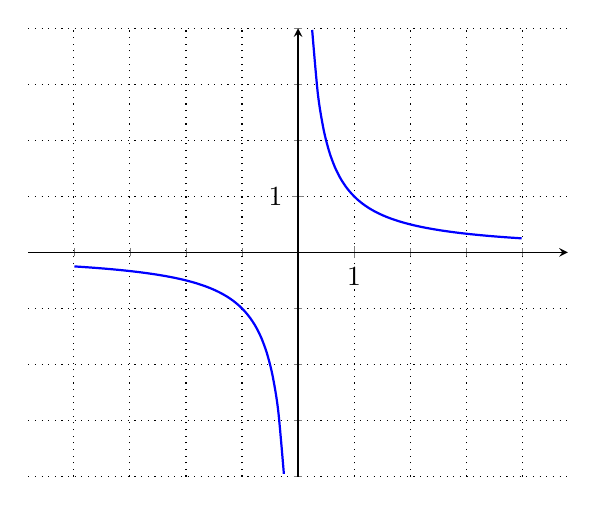
\begin{tikzpicture}
    \begin{axis}[
        axis equal,
        xtick={0,1},
        ytick={0,1},
        minor xtick={-4,-3,...,4},
        minor ytick={-4,-3,...,4},
        xmin=-4,
        xmax=4,
        ymin=-4,
        ymax=4,
        axis lines=middle,
        grid style={dotted,black},
        grid=both,
        restrict x to domain=-4:4,
        restrict y to domain=-4:4,
      ]
        \addplot [blue,thick, samples=100, smooth] {1/x)};
    \end{axis}
  \end{tikzpicture}
  \end{center}
\end{propriete}

\begin{propriete}
  Soient $a$ et $b$ deux réels non nuls.
  \begin{itemize}
    \item Si $a$ et $b$ sont négatifs, et $a\leq b$, alors $0>\frac{1}{a}\geq\frac{1}{b}$.
    \item Si $a$ et $b$ sont positifs, et $a\leq b$, alors $\frac{1}{a}\geq\frac{1}{b}>0$.
  \end{itemize}
\end{propriete}

\section{Fonctions homographiques}

\begin{definition}
  Étant donnés des réels $a$, $b$, $c$, $d$, où $c\neq0$, on appelle \emph{fonction homographique} la fonction définie sur son ensemble de définition par $f(x)=\frac{ax+b}{cx+d}$.
\end{definition}

\begin{propriete}
  Une fonction homographique $f(x)=\frac{ax+b}{cx+d}$ est définie sur $\mathbb{R}\backslash\left\{-\frac{d}{c}\right\}$
\end{propriete}

\begin{methode}
  Pour déterminer le signe d'une fonction homographique, on détermine le signe du numérateur et du dénomirateur, puis on fait un tableau de signe.
\end{methode}
\begin{exemple}
  Déterminons le signe de la fonction définie sur
  $\mathbb{R}\backslash\left\{\frac{1}{2}\right\}$ par
  $f(x)=\frac{-5x-3}{2x-1}$.

  \begin{center}
  \begin{tikzpicture}
    \tkzTabInit[espcl=3]{$x$ /1, $-5x-3$ /1, $2x-1$ /1, $\frac{-5x-3}{2x-1}$/1 }%
    {$-\infty$ ,$-\frac{3}{5}$ , $\frac{1}{2}$, $+\infty$}%
    \tkzTabLine{,+,z,-,t,-}
    \tkzTabLine{,-,t,-,z,+}
    \tkzTabLine{,-,z,+,d,-}
  \end{tikzpicture}
\end{center}
Donc $f$ est positive sur $\left[-\frac{3}{5};\frac{1}{2}\right[$, et négative sur $\left]-\infty; -\frac{3}{5}\right]\cup\left]\frac{1}{2};+\infty\right[$
\end{exemple}

\section{Équation et inéquation quotient}

\begin{propriete}
  Soit une fonction homographique $f(x)=\frac{ax+b}{cx+d}$ ($c\neq0$). La fonction $f$ est nulle si et seulement si $ax+b=0$ et $cx+d\neq0$.
\end{propriete}

\begin{propriete}
  Soit une fonction homographique $f(x)=\frac{ax+b}{cx+d}$ ($c\neq0$). La fonction $f$ est positive si et seulement si $ax+b$ et $cx+d$ sont de mêmes signes, et $cx+d\neq0$.
\end{propriete}
